\documentclass{article}
\usepackage[utf8]{inputenc}
\usepackage{amsmath}
\usepackage{graphicx}
\usepackage[T1]{fontenc}
\usepackage[french]{babel}
\usepackage{caption} 
\usepackage{amssymb}
\usepackage{float}
\usepackage{rotating,booktabs}  %rotation of table 
\usepackage[table,xcdraw]{xcolor}   % If you use beamer only pass "xcolor=table" option, i.e. \documentclass[xcolor=table]{beamer}


\title{Segmentation of contagion zones \\ in New York State}
\author{Fanirisoa Rahantamialisoa}




\begin{document}
\maketitle
   \begin{center}
   
\includegraphics[width=0.4\textwidth]{Specialization}
   \end{center}

\section{Introduction}

\subsection{Background}
COVID-19 has turned into a global crisis, evolving at unprecedented speed and scale. It is creating a universal imperative for governments and organizations to take immediate action to protect their people. 

\subsection{Problem}
One of the most important properties of epidemics is their spatial spread, a characteristic which mainly depends on the epidemic mechanism and human mobility. In this study, we are developing a geospatial and spatio-statistical analysis of the geographic dimension of the 2019 coronavirus disease pandemic (COVID-19) in New York state. The restrictions put in place to limit the diffusion and impacts of Covid-19 have had a widespread impact on people’s lives.

\subsection{ Interest}
The aim of this study is to investigate a geographic and geospatial analysis to understand the locations and distribution patterns of COVID-19 in order to be able to define and segment the zones of contagion. The study seeks to highlight the mobility dynamics of the urban population as the process of leaving from home, traveling to and from the activity locations, and engaging in activities the urban transportation system may alter the fundamental dynamics of the infectious disease, change the number of secondary infections, promote the synchronization of the disease across the city, and affect the peak of the disease outbreaks.

\section{Data acquisition and cleaning}
In this report we mostly focus our attention on New York state.  The poject collects, analyses and uses a variety of data from multiple sources. The main types of
counties that are collected and managed include :
\begin{itemize}
\item Geographic  informations for each county,
\item Metrics and indicators for each groupe of venus inside county,
\item  Official Statistical data on the COVID19 situation in each county.\\
\end{itemize}

As the sources used to collect such data are heterogeneous and diverse in nature, an Extract-Transform Load (ETL ) process is needed in each case to extract the raw data from the respective source and transform them appropriately to the corresponding representation and schema needed for being used into the analysis.\\


More specifically, a collection of ETL scripts has been designed and implemented for
cleaning,  converting and importing all collected datasets into the project repository. In general, this process proceeds in the following successive stages:
\begin{itemize}
\item \textbf{Extract data} :  mainly, three types of cases can be
distinguished, requiring different methods with varying levels of difficulty: 
\begin{enumerate}
\item US Zip Code Latitude and Longitude (using Webscraping)
\item Foursquare location data,
\item Statistical data on the COVID19 situation  (using Webscraping).
\end{enumerate}
\item  \textbf{Transform data }to fit internal representation format and schema. This stage involves selecting attributes, joining or aggregating information from multiple
records, splitting/merging values from attributes, etc.
\item  \textbf{Load data} into the repository. At this stage, previously transformed data are imported into the repository. This involves updating or replacing existing information with more recent one.\\
\end{itemize}
Such ETL operations for collecting data into  repository were implemented as custom, parametrized scripts written in Python,  developed specifically to manipulate each type of information.   If wished for, our codes can be made available on Github to wider audience.  In the rest of this section, we list the different types of data that have been collected and imported.
\subsection{Geographical Zones}
A custom Python script is used to extract by using Webscraping  from US Zip Code Latitude and Longitude and to load the records into table zones in pandas dataframe:
\begin{figure}[h]
 \centering
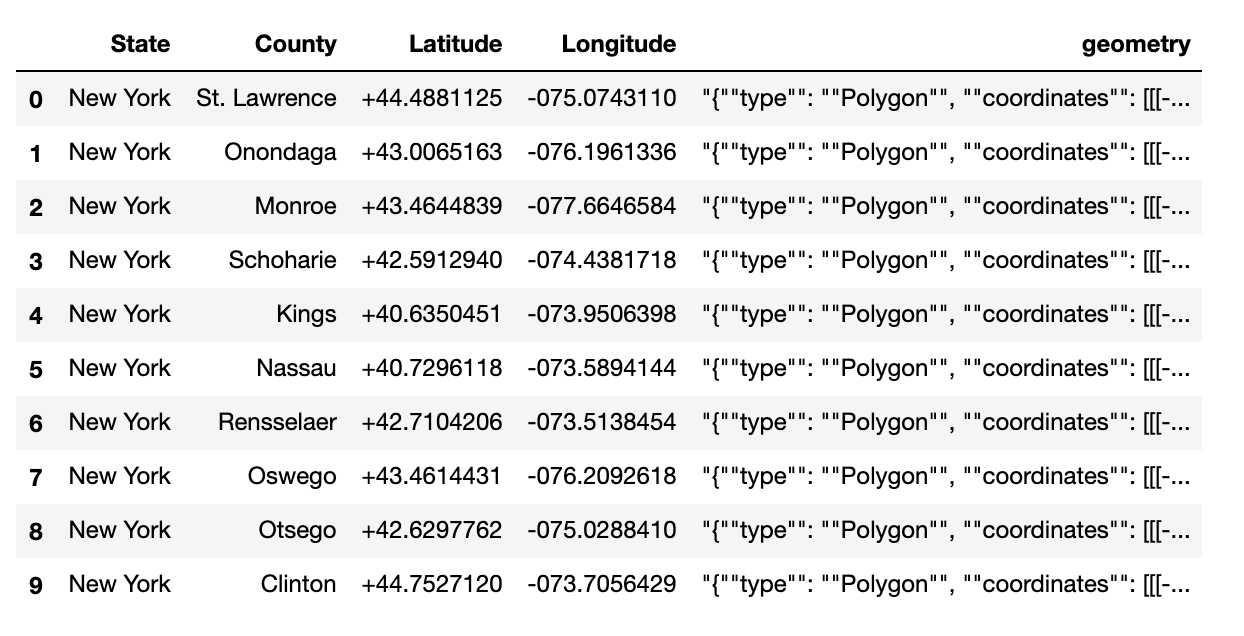
\includegraphics[width=0.75\textwidth]{geodata.png}
 \caption{US Zip Code for New York County:}
\end{figure}

As illustrated in  Figure 2 , this dataset contains 62 counties polygons :
\begin{figure}[h]
 \centering
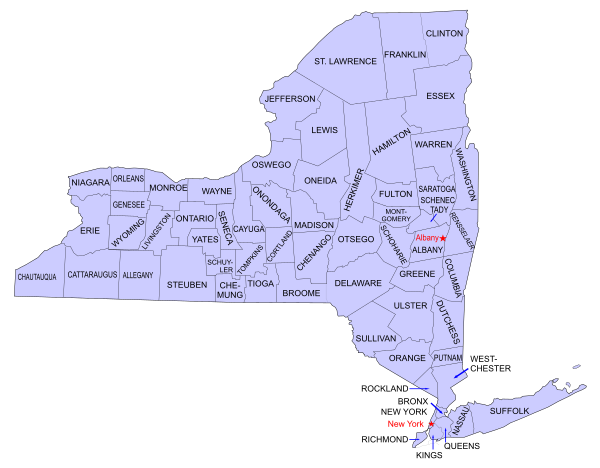
\includegraphics[width=0.7\textwidth]{NY.png}
 \caption{Counties of New York.}
\end{figure}

\subsection{Metrics for each Zones}
Extract from foursquare,  as informations and metrics,  we consider : 
\begin{itemize}
\item the number of bus stops and metro stations (the more trips, the greater the risk of transmission),
\item the number of cinemas (the more gatherings, the greater the risk of transmission),
\item the number of schools (children are vectors of transmission),
\item the number of hospitals,
\item the number of shopping centers.
\item tips : contains the total count of tips and groups with friends and others as groupTypes. Groups may change over time.
\item like : the count of users who have liked this venue, and groups containing any friends and others who have liked it. The groups included are subject to change.
\item rating : numerical rating of the venue (0 through 10). Returned as part of an explore result, excluded in search results. Not all venues will have a rating.\\
\end{itemize}

As illustrate in the Figure 3,  We obtain a dataframe  with 62 rows and 19 variables.
\begin{figure}[h]
 \centering
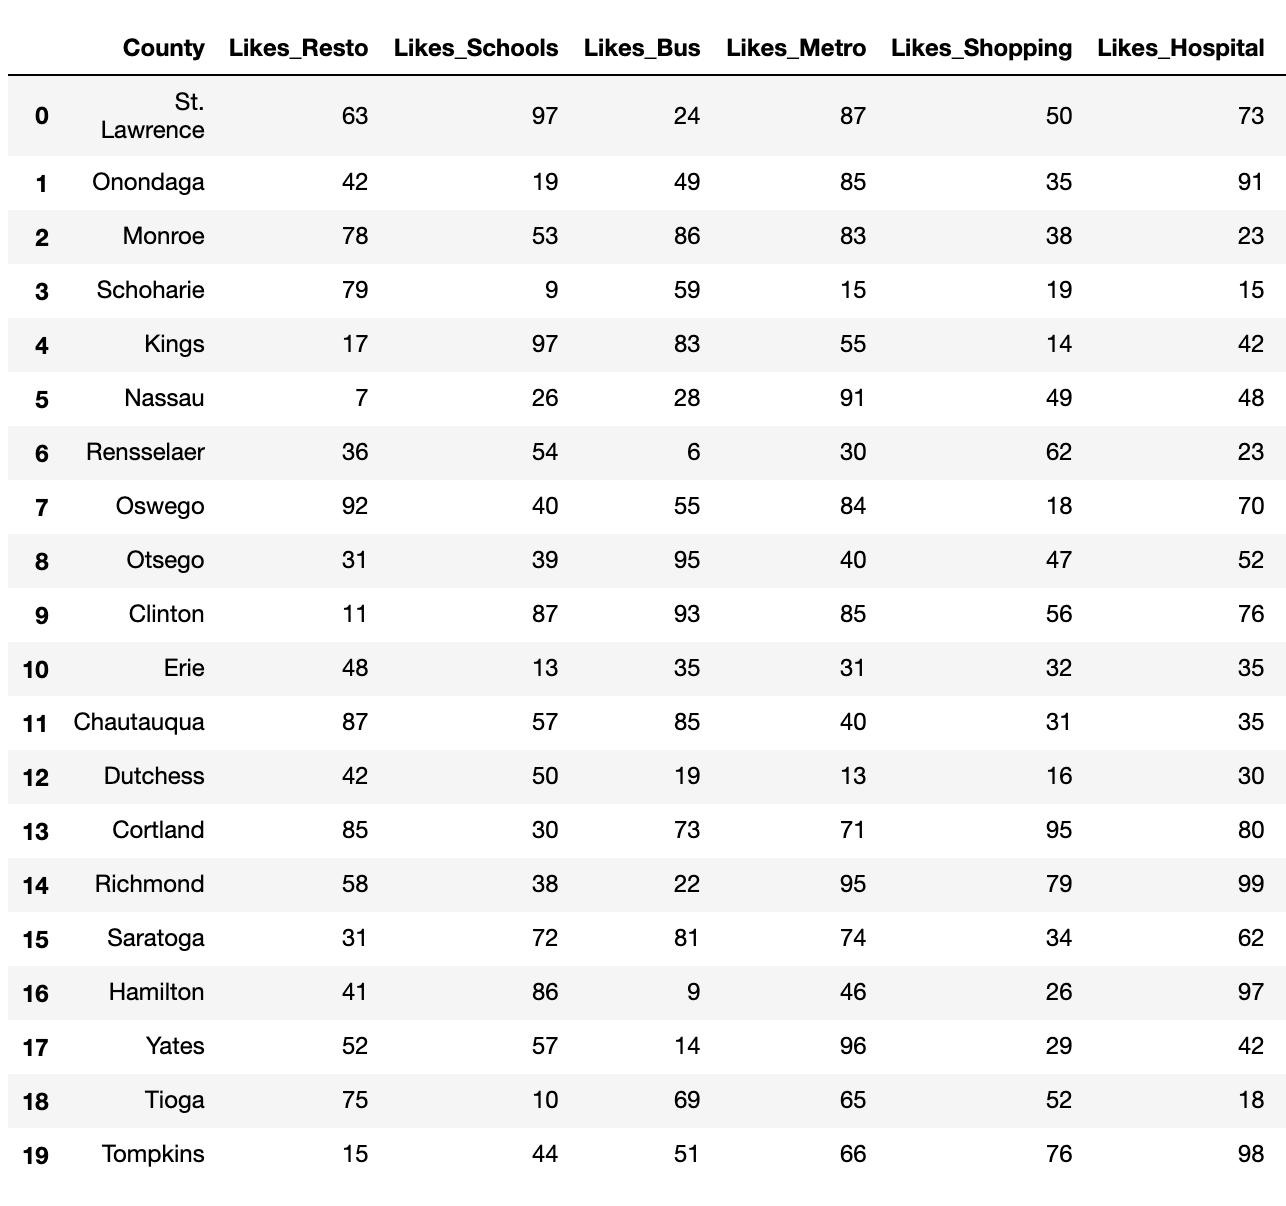
\includegraphics[width=0.8\textwidth]{metric.png}
  \caption{Counties of New York.}
\end{figure}



\subsection{Statistical data on the COVID19 }
Imports updated statistical data on the COVID19 situation in each county in Mai 2020 and September 2020: number new contaminates (J-1),
number of deaths and number of cases :
\begin{itemize}
\item Cases : The cumulative number of confirmed human cases reported to date. The actual number of infections is likely to be higher than reported.
\item Deaths : The cumulative number of confirmed human deaths reported to date. Reporting criteria vary between locations.
\item Recov : The cumulative Total of Recovered. May not correspond to actual current figures and not all recoveries may be reported.
\item Pop : The total population of the county reported to date.
\item Cases 100k : The Ratio of cumulative number of confirmed human cases reported per 100.000 population.
\item Deaths 100k : The Ratio of cumulative number of confirmed human deaths reported per 100.000 population.
\item Ratio Deaths Cases : The Ratio between cumulative number of cases and cumulative number of cases deaths.
\end{itemize}
Data will be obtained from Webscraping,  we obtain a dataframe  with 62 rows and 8 variables.
\begin{figure}[h]
 \centering
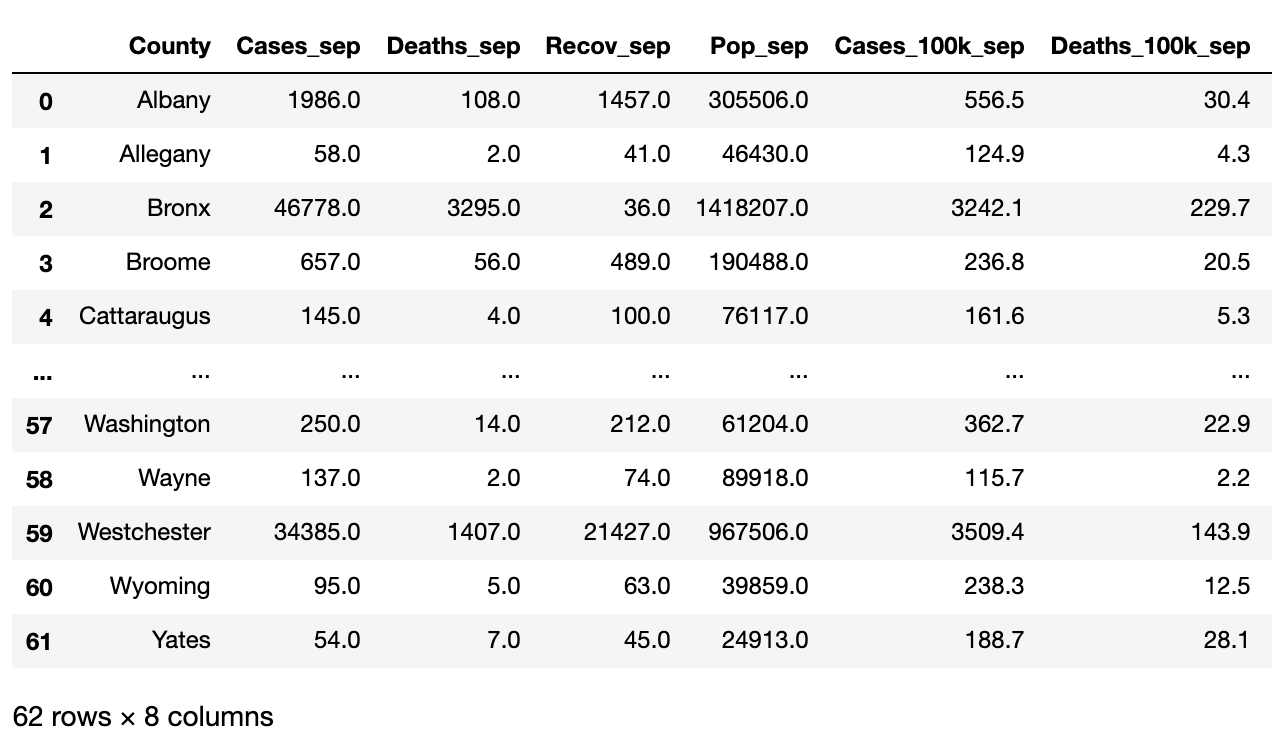
\includegraphics[width=1\textwidth]{statistic1.png}
  \caption{Statistical data on the COVID19 may 2020.}
\end{figure}

A common practice is to normalize the values of each feature before using them for clustering.  Accordingly
we use MinMaxScaler, included in the scikit-learn. This computes the minimum and maximum value of each attribute in the training set, and uses these to normalize all values in the training and the test set to the $[0, 1]$ range. In our case, the values of many features are extremely skewed;

\section{Exploratory Data Analysis}

\subsection{Number of like for restaurant \& place for  shopping}
The current growth of the fashion factory outlets results in the establishment of restaurants and cafes to capture these outside visitors.   The relationship between the two variables is not so obvious across all counties as illustrate in the following Figure:
\begin{figure}[h]
 \centering
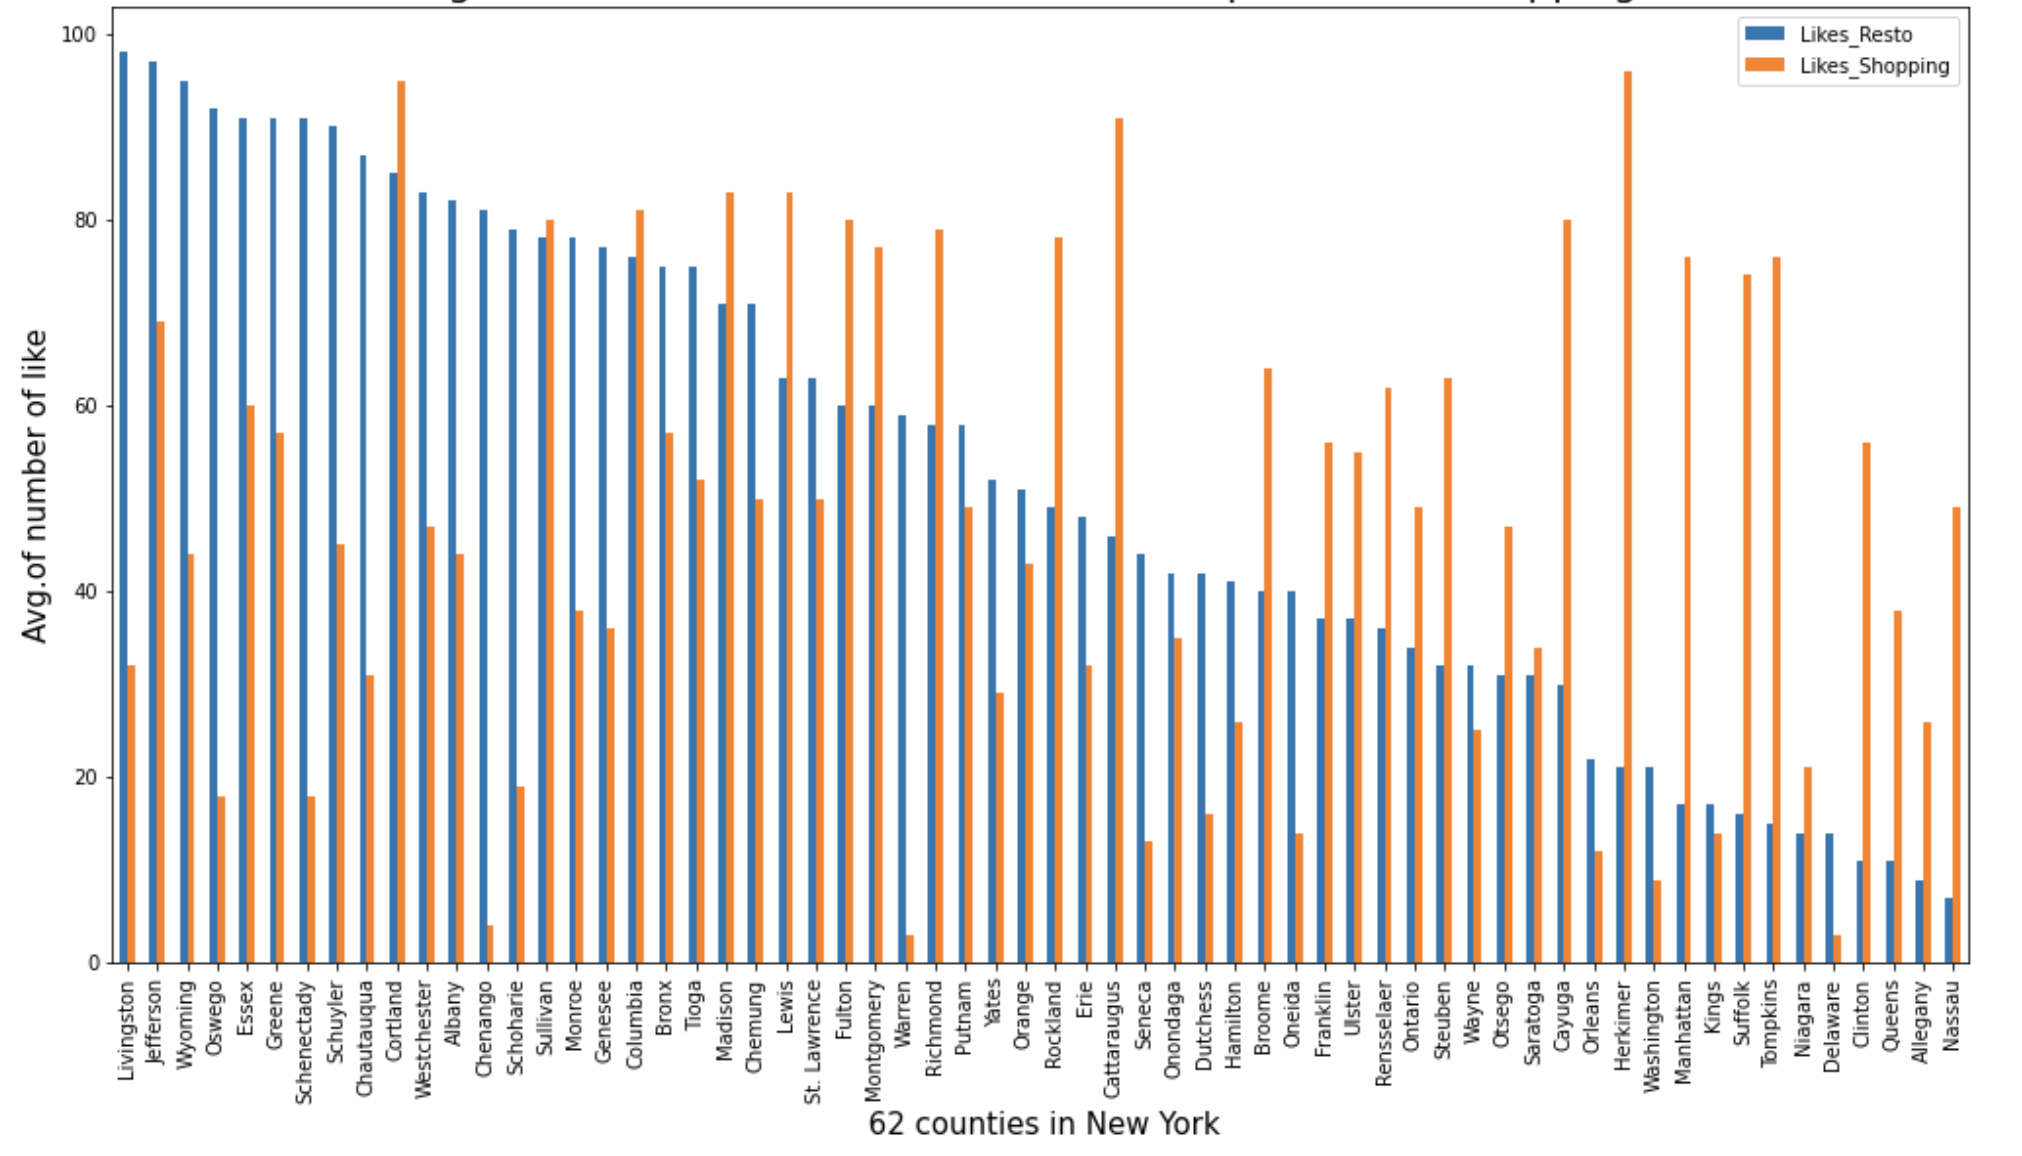
\includegraphics[width=1.06\textwidth]{compare1.png}
  \caption{Average of number of like for restaurant and place for shopping.}
\end{figure}


\subsection{Number of cases in May 2020 \& in September 2020}

About $42  \%$ of New York State residents live in New York City, so COVID stats for the entire state will tend to mirror the city's stats. This is true for positivity, which shows the same large increase in April when testing was limited, and for total tests, which have risen steadily since then. However, when looking at positive tests, you see that during the second wave, the state suffered a more pronounced rise than the city, because of large second-wave outbreaks in upstate counties. Similarly, the increase in hospitalizations and deaths in New York State is more pronounced than in New York City, because of these upstate outbreaks.\\


Queens and Brooklyn have larger populations than the other boroughs, so they tend to have more cases, but when normalized for population, Staten Island and the Bronx have often seen more positives each week. This is particularly true during the second wave, with Staten Island outstripping the other boroughs.\\


The statistics obtained over time on the numbers of cases and deaths due to the pandemic, highlight an explicit link between the number of deaths in May 2020 and the number of  cases in September 2020.   This pattern is more explicit between the numbers of  deaths recorded in May and September 2020 as illustrated by the  Figure 6. 
\begin{figure}[h!]
 \centering
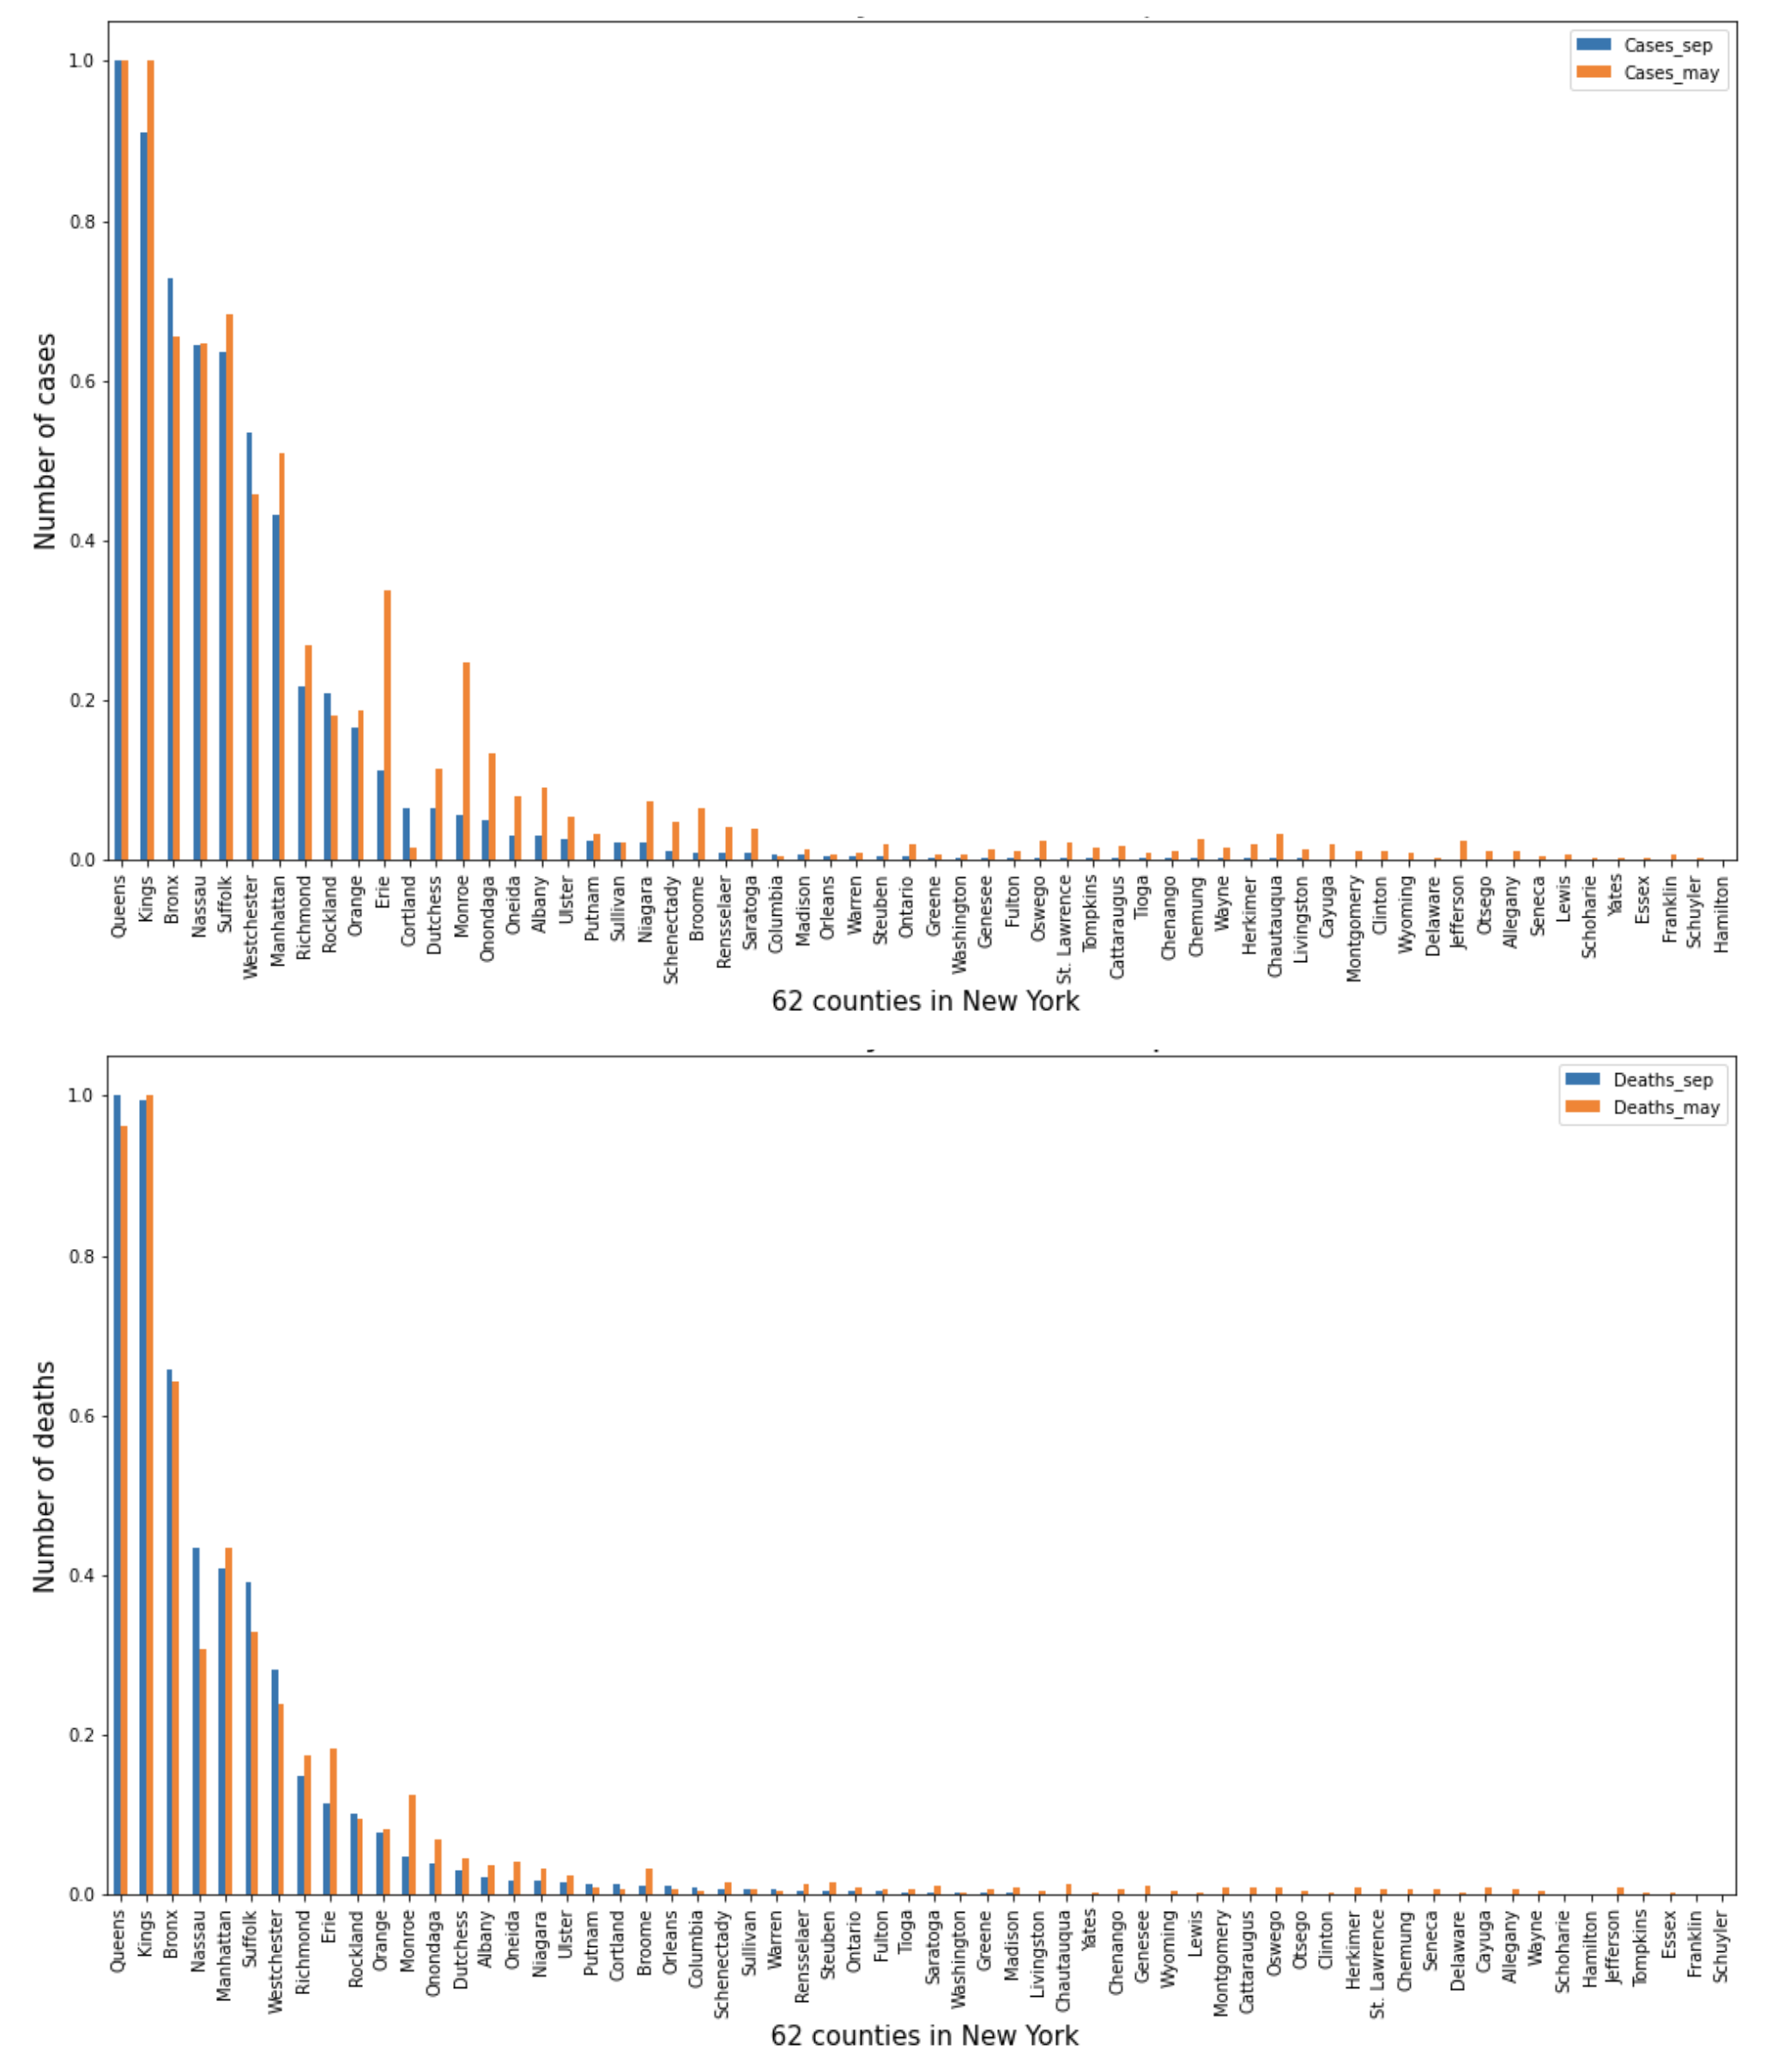
\includegraphics[width=1.06\textwidth]{compare4.png}
  \caption{Number of cases and deaths in may 2020 and in september 2020.}
\end{figure}

\subsection{Cases, deaths density per $km^{2}$  \& population density per $km^{2}$}
We used a Bubble Plot  to highlight the relationship between the number of confirmed cases,  the number of deaths and the number of population per km2 :
\begin{figure}[h!]
 \centering
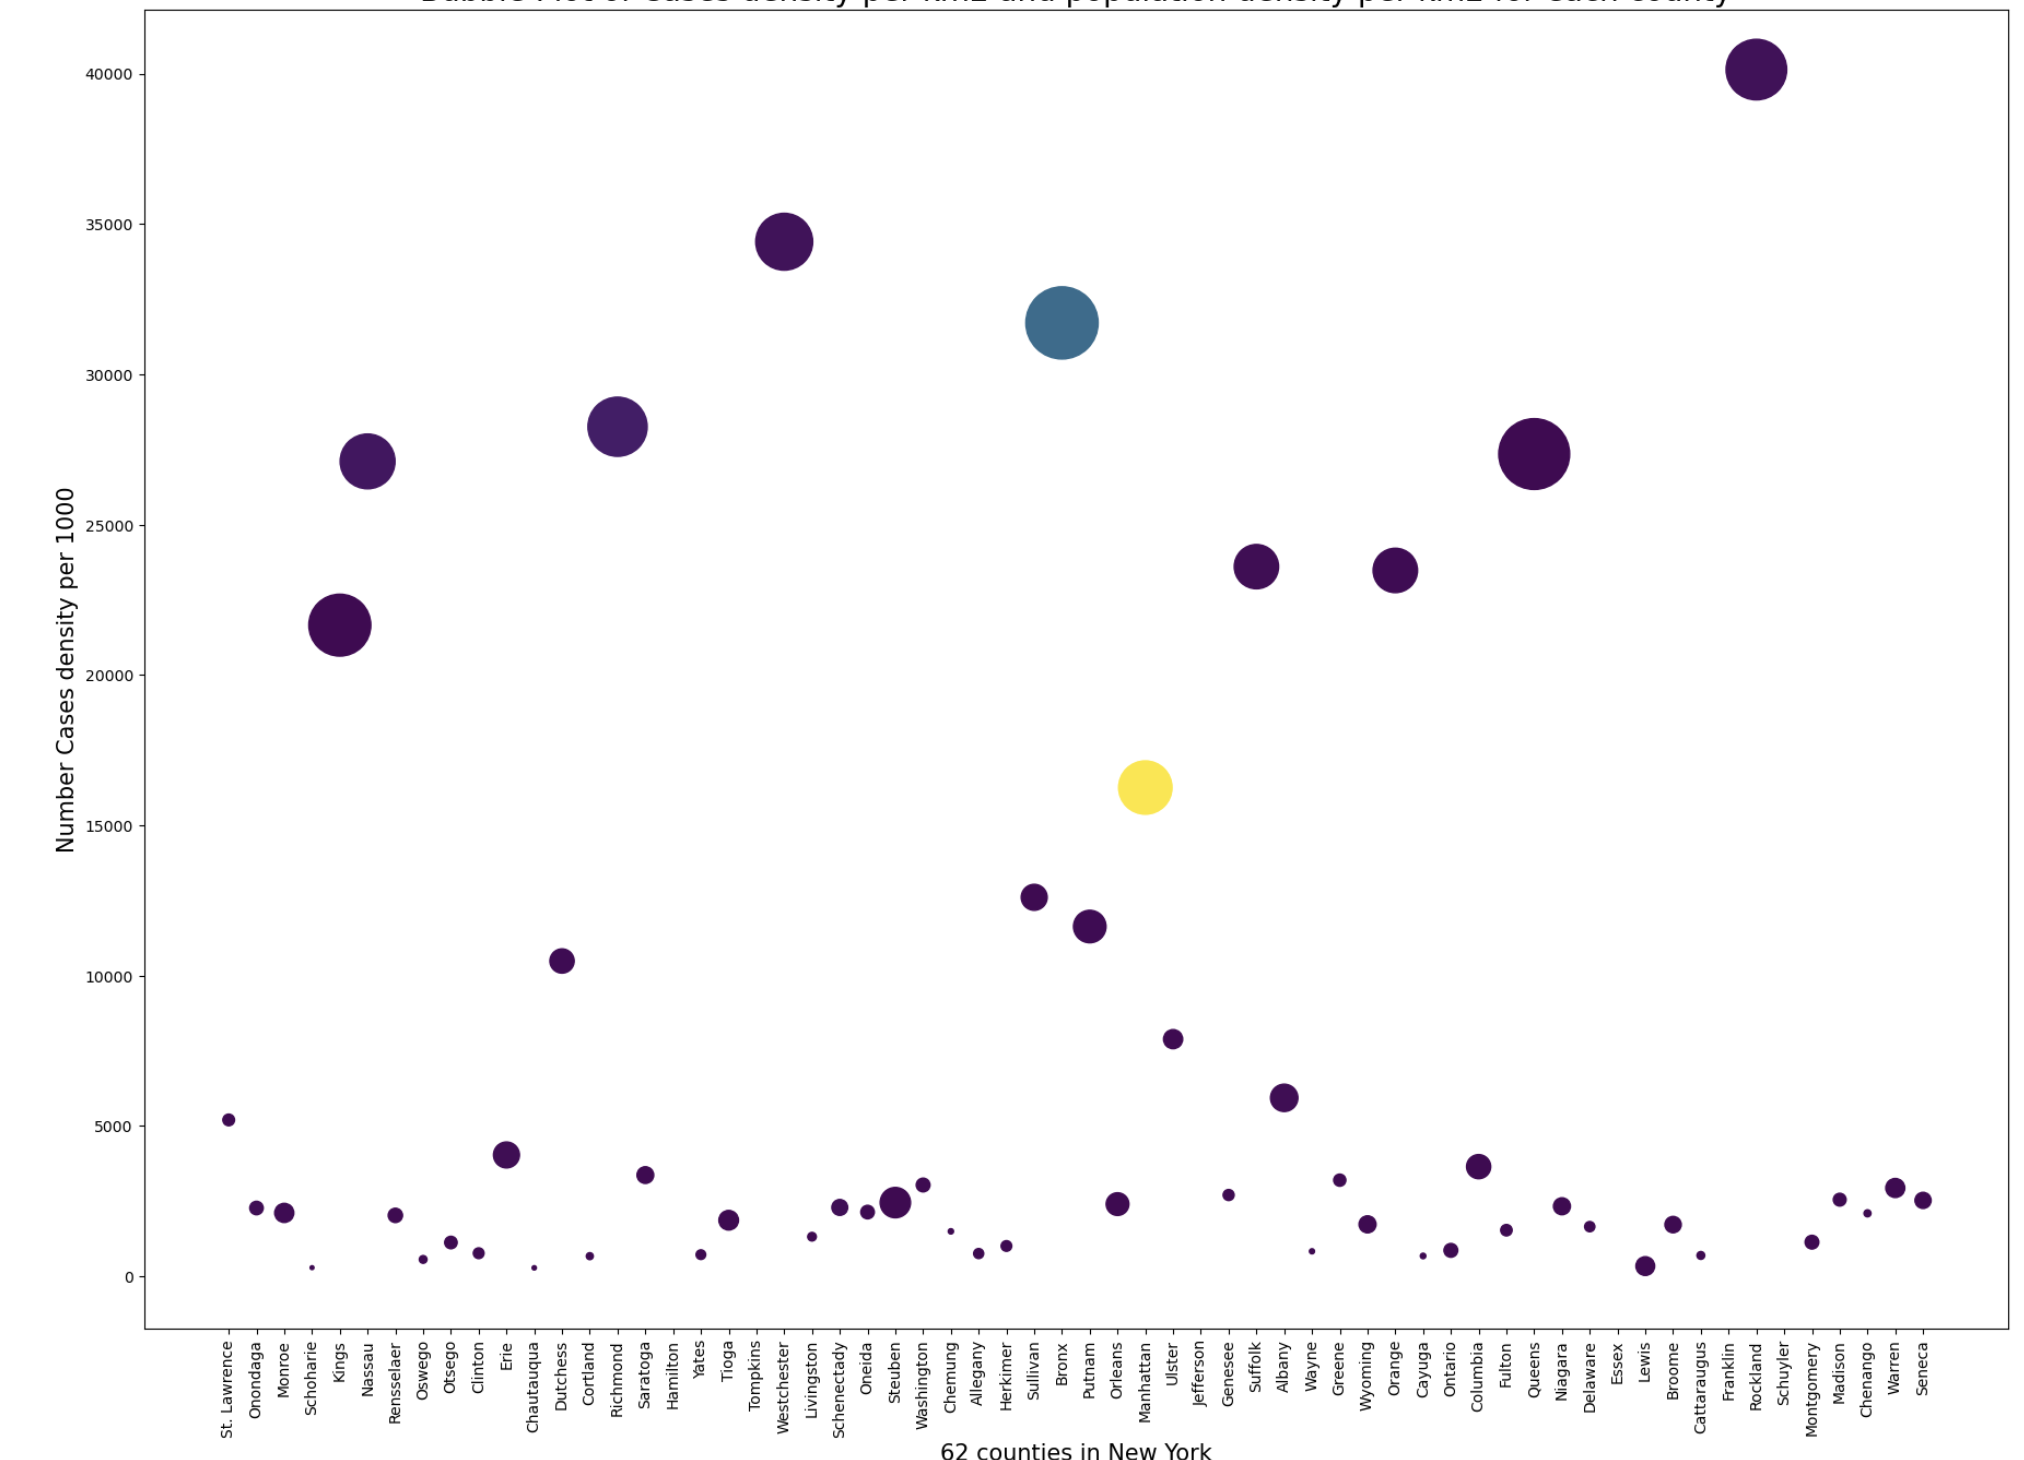
\includegraphics[width=1.06\textwidth]{compare5.png}
 \caption{Bubble Plot of Cases,  death density per km2 and population density per km2 for each county.}
\end{figure}

The result does not make it possible to directly highlight the relationship between the 3 dimensions of confirmed cases, recorded deaths and number of population per km2. In the figure, we have the size of the sphere which represents the number of deaths, and the color the number of population.

\section{Analysis of Zone-Based Clustering}
Under these updated metrics,  the goal is to Identify the set of objects with similar characteristic.  Clustering can be considered the most important unsupervised learning problem; so, as every other problem of this
kind, it deals with finding a structure in a collection of unlabeled data.
Micro-cluster zones will now be determined using K-means.\\

We can build the K-Means in python using the KMeans algorithm provided by the scikit-learn package. The KMeans class has many parameters that can be used, but we will be using these three:

\begin{itemize}
\item Init : Initialization method of the centroids. The value will be: $k-means++ $ Selects initial cluster centers for the $k-means$ clustering in a smart way to speed up convergence..
\item $n_clusters$ : The number of clusters to form as well as the number of centroids to generate. The value will be 5
\item $n_init$ : Number of times the k-means algorithm will be run with different centroid seeds
\end{itemize}

The final results will be the best output of $n_init$ consecutive runs in terms of inertia.  The value will be $12$ After building the model, we will be fitting and define a variable ‘labels’ to store the cluster labels of the built model. Let’s do it in python.   The  class of  cluster for each county are represented inn the following :
\begin{figure}[h!]
 \centering
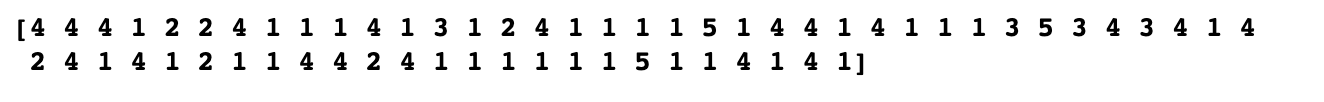
\includegraphics[width=1.06\textwidth]{resulte.png}
 \caption{The  result of the K-means clustering analysis for all the 62 counties.}
\end{figure}

According to Figure 9, it can be found that as the value of k equal to 5.

\begin{figure}[h!]
 \centering
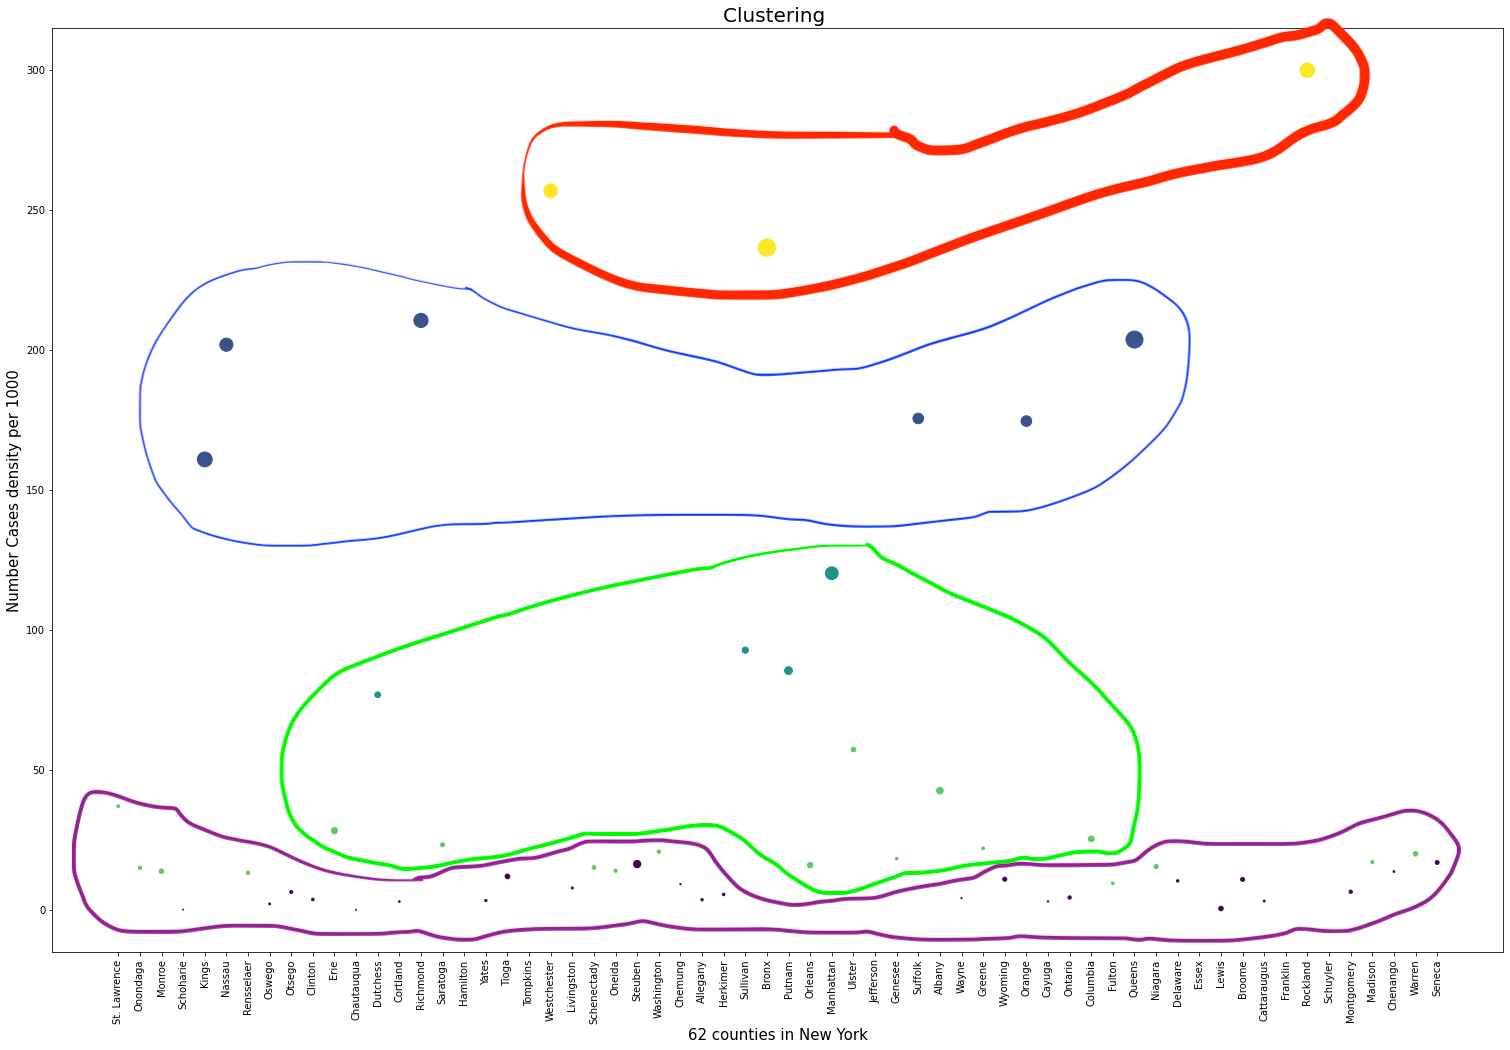
\includegraphics[width=0.9\textwidth]{kmeans2.png}
 \caption{The  result of the K-means clustering analysis for all the 62 counties.}
\end{figure}

A clustering-based approach can be used to solve the problems. Clustering involves grouping of similar elements of a given set of elements. By analyzing the clusters, we discover common or discriminative factors among the clusters that are likely to explore whether clusters of contacts could better explain the transmission of infectious diseases.\\

The results of clustering are highly dependent on the features used. The result reveals that 5 region clusters were created from 62 counties, represented using different colors. Generally, geographically adjacent regions were more likely to be grouped into the same cluster. This result is consistent with previous studies. However, we did not find significant differences between clusters, unlike the disease-based clusters or time-based clusters. That is, the difference in the occurrence of infectious diseases was too small to separate into clusters.

\section{Conclusion}
The k-means algorithm is a well-known partitional clustering algorithm. But the traditional approach selects the number of clusters (k), prior to the clustering process, and randomly selected initial centroids to produce the clusters. Since the initial centroids which is selected randomly will contribute much on the accuracy of this clusters, accuracy cannot be guaranteed.


\end{document}
